\documentclass[a4paper,12pt]{article}
\usepackage[osf]{mathpazo}
\usepackage{ms}
\usepackage[numbers, sort&compress]{natbib}
\usepackage{lineno}
\usepackage{graphicx}
\usepackage{caption}
\modulolinenumbers[5]
\linenumbers

\pdfminorversion=3

\makeatletter
\renewcommand{\@biblabel}[1]{\quad#1.}
\makeatother

\title{The adequacy of phylogenetic trait models}
\author{
Matthew W. Pennell$^{1, *}$, Richard G. FitzJohn$^2$,\\
William K. Cornwell$^{3}$ \& Luke J. Harmon$^{1,4}$
}

\date{}
\affiliation{
 $^{1}$ Department of Biological Sciences \& Institute for Bioinformatics and Evolutionary Studies, University of Idaho, Moscow, ID 83844, U.S.A.\\ 
 $^{*}$ Email for correspondence: \texttt{mwpennell@gmail.com}\\
 $^{2}$ Department of Biological Sciences, Macquarie University, Sydney, NSW 2109, Australia;
\texttt{rich.fitzjohn@gmail.com}\\
 $^{3}$ School of Biological, Earth and Environmental Sciences, University of New South Wales, Sydney, NSW 2052, Australia; \texttt{w.cornwell@unsw.edu.au}\\
 $^{4}$ \texttt{lukeh@uidaho.edu}
}

\runninghead{are macroevolutionary models adequate?}
\keywords{comparative methods, model adequacy, independent contrasts, Brownian motion}


\begin{document}

\mstitlepage
\parindent=1.5em
\addtolength{\parskip}{.3em}
\vfill

\singlespacing
\section{Abstract}
Phylogenetic thinking is now pervasive in biology. Researchers from a variety of fields are increasingly using phylogenetic comparative methods (PCMs) to test evolutionary hypotheses using interspecific data.  PCMs requires both a phylogeny and a statistical model that describes the evolution of the trait through time.
A wide variety of such models have been proposed, all of which necessarily make
simplifying assumptions. In selecting a model, researchers have relied, almost exclusively, on measures of relative fit. Disconcertingly, we currently have no way of knowing if any of the models used in comparative biology provide good explanations for the data. Here we address two outstanding questions in comparative biology. First,
we develop a general framework for assessing the absolute fit (or, adequacy) of quantitative trait models, based on Felsenstein's Independent Contrasts method. Our framework can be applied to arbitrarily complex quantitative trait models. We then use our approach to assess whether commonly used models are reasonable descriptors of the macroevolutionary dynamics of three important angiosperm functional traits. We find that model fit is surprisingly poor; this is true across many clades and at multiple time scales. This result has serious implications for both developers of comparative methods and studies that make use of them. We argue that assessment of model adequacy should become a routine component of phylogenetic comparative studies.

\vfill

\newpage



\begin{quotation}
\noindent There are known knowns; there are things we know we know. There are known unknowns; that is to say, there are things that we now know we don't know. But there are also unknown unknowns --- there are things we do not know we don't know.

---Fmr. U.S. Secretary of Defense Donald Rumsfeld
\end{quotation}

\section{Introduction}
Nothing in biology makes sense except in light of phylogeny. Phylogenetic trees and phylogenetic thinking are ubiquitous in modern biology \citep{PennellHarmon}; ecologists, geneticists, paleontologists and anthropologists now widely recognize that a historical perspective can provide novel insights into evolutionary questions. This interest in phylogenetic biology has risen in lockstep with developments in phylogenetic comparative methods (PCMs; reviewed in \citep{PennellHarmon}). 

Modern PCMs are almost exclusively model--based, meaning inferences are contigent on both the phylogenetic tree and the chosen probabilistic model. Selecting a good model is therefore essential for making robust inferences. Model choice should be guided by several considerations. One is interpretation: does the model capture the processes relevant to the question \citep{HansenOrzack2005, Hansen2012, PennellPE}? Another, the focus of this paper, is statistical: does the model provide a good explanation for the dataset? In phylogenetic comparative biology, this latter question has been addressed, almost exclusively, by comparing the relative fit of a number of models and selecting the best one for inference \citep{Mooers1999, Harmon2010, Hunt2012}. 

But the relative support for a model is only a partial answer to the question of whether it is a good explanation for the data. It is also important to consider whether the model is a good fit, or adequate, on its own terms. The best of a poor set of models is still a poor model. Assessing model adequacy is a routine step in many statistical applications, especially Bayesian statistics \citep{Gelmanbook}. Failure to check model adequacy can potentially result in erroneous inferences. A classic example of this in molecular systematics is the disputed phylogenetic relationships of rodents. A number of early molecular phylogenetic studies reported evidence that ``strongly contradict[ed]'' the traditional hypothesis that the order Rodentia is a monophyletic group \citep{Graur1991, DErchia1996}. Sullivan and Swofford \citep{SullivanSwofford} demonstrated that these conclusions were misleading, and resulted entirely from using models of molecular evolution that did not adequately accomodate  heterogeneity in rates of evolution across sites. There are many similar case--studies throughout and outside of evolutionary biology.

Many models for describing the evolution of phenotypic traits along a phylogeny have been developed, as well as sophisticated machinery for fitting them to data (e.g., \citep{Felsenstein1985, Hansen1997, Pagel1999, Blomberg2003, ButlerKing2004, Omeara2006, Eastman2011, Beaulieu2012, SlaterMEE, UyedaBayou}). Using these models, researchers from across biological disciplines have made exciting discoveries that would not have been possible without a phylogenetic perspective. However, it is disconcerting that we generally have no idea if the models used in PCMs are adequate; there are no general procedures that can be used to assess the adequacy of all of the models referenced above. Even more troubling is that model adequacy is rarely ever considered when PCMs are applied. To borrow Rumsfeld's taxonomy, model adequacy has largely been an ``unknown unknown'' in PCMs.

In this paper we seek to (at least somewhat) rectify this situation. We address two major outstanding problems in comparative biology. First, we develop a general framework for assessing the adequacy of phylogenetic models of trait change, specifically those for quantitative characters. Second, we assess the adequacy of simple models of trait evolution across scales, using a recently published mega--phylogeny of Angiosperms (flowering plants) \citep{Zanne2013} and data on three important functional traits --- specific leaf area, seed mass, and leaf nitrogen content --- compiled from the literature. 

\section{A general framework for assessing model adequacy}
The basic concept of our approach is straightforward. We have a phylogenetic tree consisting of $n$ lineages. We have data on the the trait values observed at each tip $X$ ($X= X_1, X_2, \ldots, X_n$). In order to make inferences from the distribution of traits at the tips, we fit a model $\mathcal{M}$, describing the evolution of the trait along the phylogeny, and estimate a set of parameters $\Theta_{\mathcal{M}}$. In most analyses using comparative data, the aim is to ask: what $\Theta_{\mathcal{M}}$  maximizes the probability of observing $X|\mathcal{M}$?; what is the posterior distribution of $\Theta_{\mathcal{M}}|X, \mathcal{M}$?; or, does $\mathcal{M}_1$ explain the data better than $\mathcal{M}_0$? Our approach is conceptually distinct in that we are asking: how likely is it that $\mathcal{M}$ would produce a dataset similar to $X$ if we re--ran evolution?

We have developed two separate ways to ask this question --- one frequentist, the other Bayesian. While these approaches are philosophically different from one another, in practice, they are very similar. In a frequentist paradigm, we can assess model adequacy by performing parametric bootstrapping. We estimate $\Theta_{\mathcal{M}}$ using maximum likelihood, restricted maximum likelihood, least--squares, etc. We then simulate new datasets $Y$ by evolving a trait along the phylogeny according to $\mathcal{M}(\Theta_{\mathcal{M}})$. We can then compare $X$ and $Y$. However, In order to make any sort of comparison, we must first summarize $X$ and $Y$ using a meaningful summary statistic or a set of summary statistics $\mathcal{S}$. If $\mathcal{S}_X$ is more extreme than most of the distribution of $\mathcal{S}_Y$, we can conclude that $\mathcal{M}(\Theta_{\mathcal{M}})$ is not a good explanation for $X$. Parametric bootstrapping is likely familiar to phylogenetic biologists in the form of the Goldman--Cox test \citep{Goldman} for the adequacy of sequence evolution models, and the Shimodaira--Hasegawa (SH) test \citep{SH} for comparing topologies. 

Alternatively, one may adopt a Bayesian perspective and estimate the posterior distribution of $\mathcal{M}$, $\mathbb{P}(\Theta_{\mathcal{M}}|X,\mathcal{M})$ using Bayes theorem
\[\mathbb{P}(\Theta_{\mathcal{M}}|X,\mathcal{M}) = \frac{\mathbb{P}(X|\Theta_{\mathcal{M}}, \mathcal{M})\mathbb{P}(\Theta_\mathcal{M}, \mathcal{M})}{\mathbb{P}(X|\mathcal{M})} \]
and Markov chain Monte Carlo (MCMC) machinery. To assess the adequacy of the model we perform posterior predictive simulations \citep{Rubin1984, Gelman1996}. The posterior predictive distribution is defined as
\[\mathbb{P}(Y|X,\mathcal{M}) = \int \mathbb{P}(Y|\Theta_{\mathcal{M}}, \mathcal{M})\mathbb{P}(\Theta_{\mathcal{M}}|X,\mathcal{M})d\Theta_{\mathcal{M}}. \]
where $\mathbb{P}(Y|X,\mathcal{M})$ is simply the probability of getting a new dataset $Y$ given $X$ and $\mathcal{M}$. We obtain this distribution by drawing repeated samples from $\mathbb{P}(\Theta_{\mathcal{M}}|X,\mathcal{M})$ and simulating datasets from the sampled parameters. We can compute the $\mathcal{S}$ over the distributions of $\Theta_{\mathcal{M}}|X,\mathcal{M}$ and $Y|\mathcal{M},X$ and compare the two. Posterior predictive simulation appraoches have also been developed for molecular phylogenetics \citep{Bollback2002, Reid2013, Lewis2013, Brown2013} but have unfortunately not been widely adopted \citep{Brown2013}.


\subsection{Summary statistics}
As stated above, in order to compare the observed data $X$ with the data simulated under the fitted model $Y$ we need some way of summarizing the observations to make meaningful comparisons. 
In our approach we calculate a set of summary statistics on the contrasts (\textit{sensu} Felsenstein \citep{Felsenstein1985}) computed at each node, rather than on the data itself. (We refer readers to \citep{Felsenstein1985, Rohlf2001, Blomberg2012}, for details on how contrasts are calculated.) Contrasts are a natural way of summarizing phylogenetically structured quantiative data with very little loss of information (lose only 1 degree of freedom). Importantly, contrasts have the useful statistical property that if Brownian motion (BM; in which the variance in the trait increases linearly at rate $\sigma^2$) is a good model for the evolution of the trait, they will be independent and identically distributed (i.i.d.) $\sim \mathcal{N}(0, \sigma)$. The raw data can only be i.i.d. if the phylogeny is not informative. 

We have chosen a set of six summary statistics $\mathcal{S} = \lbrace \mathcal{S}_1, \ldots, \mathcal{S}_6 \rbrace$ to compute on the contrasts of both our observed data and our simulated data.

\begin{enumerate}
\item[$\mathcal{S}_1$] The mean of the squared contrasts. This is equivalent to the restricted maximum likelihood (REML) estimator of the Brownian motion rate parameter $\sigma^2$ \citep{Garland1992, Rohlf2001}. $\mathcal{S}_1$ is a used as a global rate estimate.

\item[$\mathcal{S}_2$] The variance in the absolute value of the contrasts. If the variance of the observed contrasts is greater than that of the simulated contrasts, it suggests that we are not properly accounting for rate heterogeneity across the phylogeny. If the variance of the observed is smaller, it suggests that trait is somehow more contrained than the model assumes.

\item[$\mathcal{S}_3$] The slope resulting from fitting a linear model between the absolute value of the contrasts and their expected variances, with the expected variances as the independent variable. Each (standardized) contrast has an expected variance proportional to the sum of the branch lengths connecting the node at which it is computed to its daughter lineages  \citep{Felsenstein1985}. Under a model of BM, we expect no relationship between the contrasts and their variances. We use $\mathcal{S}_3$ to test if contrasts are larger or smaller than we expect based on their branch lengths. If, for example, more evolution occured per unit time on short branches than long branches, we would observe a negative slope.

\item[$\mathcal{S}_4$] The slope resulting from fitting a linear model between the absolute value of the contrasts and the inferred ancestral state, with the inferred ancestral states as the independent variable. We estimated the ancestral state using the least--squares method suggested by Felsenstein \citep{Felsenstein1985} for the calculation of contrasts. We note that this is not technically an ancestral state reconstruction (see \citep{Felsenstein1985}); it is more properly thought of as a weighted average value. We used this statistic to evaluate whether there is variation in rates relative to the trait value (e.g., do larger organisms evolve proportionally faster than smaller ones?)

\item[$\mathcal{S}_5$] The slope resulting from fitting a linear model between the absolute value of the contrasts and the height of the node at which they are inferred measured from the root, with the node height as the independent variable. This is used to capture variation relative to time. It is alternatively known as the ``node--height test'' \citep{FreckletonHarvey2006, SlaterPennell} and used for detecting early bursts of trait evolution during adaptive radiations. 

\item[$\mathcal{S}_6$] The D--statistic obtained from Kolmolgorov--Smirnov test from comparing the distribution of contrasts to that of a normal distribution with mean 0 and standard deviation equal to the root of the mean of squared contrasts (the expected distribution of the contrasts under BM; see \citep{Felsenstein1985, Rohlf2001}). We chose this to capture deviations from normality. For example, if traits evolved via a ``jump--diffusion'' type process \citep{Landis2012}, in which there were occasional large ``jumps'' in phenotypic space \citep{PennellPE}, the tip data would no longer be multivariate normal owing to a few contrasts throughout the tree being much larger than the rest. 

\end{enumerate}

We have chosen these six summary statistics because they capture a range of dimensions of variability wherein the model may not be adequate. However, they are certainly not exhaustive. One could, for instance, calculate the median of the squared contrasts, the skew of the distribution of contrasts, etc. If the generating model was known, we could use established procedures for selecting a set of sufficient (or, approximately sufficient \citep{MajoramJoyce}) summary statistics for that model. However, the aim of our approach is assess the fit of the model without reference to a true model. Our chosen statistics capture a wide variety of model misspecifications but this does not mean that they will necessarily capture every type of model misspecification. Researchers interested in specific questions are encouraged to use alternate sets of summary statistics. The choice of what summary statistics to use is ultimately one of balancing statistical intuition and computational effort. Unfortunately, there is no good statistical theory to guide us as to which summary statistics to use and how many are enough \citep{Gelmanbook}.

\subsection*{Generalizing the approach}

All of the summary statistics essentially evaluate the condition that the contrasts are i.i.d. and come the expected distribution. If we assume that the data has arisen as a result of a BM--like process and this condition does not hold, the model can be rejected as inadequate. Our summary statistics $\mathcal{S}_3$, $\mathcal{S}_4$, and $\mathcal{S}_5$ have been used previously in the literature with this justification \citep{Garland1992, Garland1993,  Diaz1996}. However, if we assume that our traits have evolved under a different model, such as an Ornstein--Uhlenbeck (OU; \citep{Hansen1997}) or a multi--rate BM model, then we no longer necessarily expect the contrasts to be i.i.d. The expected distribution of contrasts under most models is not characterized and even if it was, this would necessitate a model--specific set of summary statistics for every model.

Our solution to this problem is to create what we term a ``unit tree'' (see Box 1). A unit tree is defined as a phylogeny which has branch lengths in units of expected (standardized) variance. We can rescale a phylogeny with branch lengths in time units to a unit tree using the parameters of any quantitative trait model, as long as the data at the tips is assumed to come from a multivariate normal distribution. This applies to nearly all models used in comparative biology \citep{Omeara2012}. If the model that is fit is the generating model, or an adequate alternative, the contrasts will be i.i.d. according to a standard normal distribution $\mathcal{N}(0,1)$. In other words, if the model is good, the trait data at the tips will have the same distribution as data generated under a BM process with a rate of 1 (hence the term ``unit tree''). Creating the unit tree from the estimated model parameters prior to computing the contrasts generalizes the summary statistics to most models of trait evolution.

Calculating the contrasts on the unit tree also means that rather than simulate trait evolution under the model, we can simulate many datasets under a BM process ($\sigma^2 =$ 1), which is computationally efficient. The distribution of summary statistics calculated on these simulated data sets can then be compared to the summary statistics from the observed data. We summarize the entire approach in Figure \ref{fig:flowchart}.

\subsection{A case study: seed size evolution in the Meliaceae and Fagaceae }
%% TODO (MWP): check all numbers used in this section.
To illustrate our approach we examine seed size evolution in two tree families, the Meliaceae (the mahogany family) and Fagaceae (which contains oaks, chestnuts and beech trees). The trait data and phylogeny for both groups are subsets of the larger dataset used in the analysis (see below). Superficially, these datasets are quite similar. Both are of similar size (Meliaceae: 44 species in dataset; Fagaceae: 70 species) and are ecologically comparable. Following Harmon et al. \citep{Harmon2010} we fit simple models of trait evolution to the data: 1) BM, which is often associated with genetic drift \citep{Lande1976, Felsenstein1988, Lynch1990, HansenMartins1996}, randomly--varying selection \citep{Felsenstein1973}, or the summation of many processes over macroevolutionary time \citep{HansenMartins1996, Uyeda2011, PennellPE}; 2) single optimum OU, which is often assumed to represent stabilizing selection (following Lande \citep{Lande1976}), though we think a more meaningful interpretation is that it represents an ``adaptive zone'' \citep{Hansen2012book, PennellHarmon}; and 3) EB, which was developed as a mathematical represenation of a niche--filling process during an adaptive radiation \citep{Harmon2010, SlaterPennell}. We computed AIC weights \citep{aicweight} for the three models and for both datasets, an OU model was overwhelmingly supported (AICw $>$ 0.98 for both groups). Using the conventional model selection approach commonly used in comparative biology, we might conclude that similar evolutionary processes are important in these two clades of trees.

Examining model adequacy provides an alternative perspective. We took the MLE of the parameters from the OU models for each dataset, constructed a unit tree based on those parameters. We calculated our six summary statistics on the contrasts of the data, then simulated 1000 BM datasets on the unit tree and calculated the summary statistics on the contrasts of each simulated dataset. The results from the analyses of model adequacy are shown in Figure \ref{fig:two-clades}. For seed size evolution in Meliaceae, the OU model selected by AIC was an adequate model; the observed summary statistics were in the middle of the distribution of simulated summary statistics ($\mathcal{S}_1: p=0.448$, $\mathcal{S}_2: p=0.803$, $\mathcal{S}_3: p=0.633$, $\mathcal{S}_4:p=0.496$, $\mathcal{S}_5: p=0.148$, $\mathcal{S}_6: p=0.629$). For the Fagaceae, the story is different. The OU model was revealed to be inadequate by both $\mathcal{S}_1$ ($p \sim 0$) and by $\mathcal{S}_2$ ($p=0.006)$; the rest of the observed summary statistics did not differ significantly from the simulated summary statistics ($\mathcal{S}_3: p=0.228$, $\mathcal{S}_4:p=0.364$, $\mathcal{S}_5: p=0.828$, $\mathcal{S}_6: p=0.955$). This example serves to illustrate the distinction between the conventional approach to model selection in PCMs and model adequacy. Selecting amongst a limited pool of models does not give a complete picture of whether a model is appopriate. We will return to this case study in this discussion.


\section{The adequacy of models for the evolution of plant functional traits}

We used the approach we developed to address an outstanding question in comparative biology: how well do commonly used models explain the evolution of traits along a phylogeny and when are more complex models required. We addressed this question by studying Angiosperm functional traits using a recently published a megaphylogeny of containing 31,749 species of seed plants \citep{Zanne2013}. This dataset is exceptional in terms of scope and allowed us to evaluate the adequacy of models through time and across many groups.  

We compiled data on three traits from the literature --- specific leaf area (SLA), seed mass and nitrogen content (see Methods for details on datasets). These are commonly used proxies for functional variation in plants (hydrodynamic cycling, life history characteristics, and photsynthetic capabilities, respectively \citep{Westoby2002}). We  matched these data to the phylogeny. We pulled out xx subclades, extracting named (family and orders) and unnamed clades taken from time--slices across the tree. As with the Meliaceae and Fagaceae (above), we fit the three models (BM, OU, EB) to each subclade. We evaluated the relative support for each of the three models using conventional model selection techniques and then assessed the adequacy of the models using our procedure. (See Methods section for further details.) 

\section{Empirical Results}

[\emph{This is the roughest part; will work on this a lot more}]:

All analyses were performed using both likelihood and Bayesian methods (see Data and Methods). For the sake of clarity, we present only the results from likelihood analyses here. Results from Bayesian inference were broadly similar and are presented in full in the Supplementary Material. Across the xx subclades, we found widespread support for OU models. For xx\% of clades, OU had $\sim$ 100\% of the AIC weight and yy\% of clades had $>$ 75\% support (Figure \ref{fig:aic-support}). Similar to the analysis of Harmon et al. \citep{Harmon2010} we found very little support for EB models (only xx\% of clades supported EB with $>$ 75\% AIC weights), suggesting that ``early bursts'' of trait evolution may indeed be rare in these datasets (but see \citep{SlaterPennell}). Larger clades were more likely to have high support for a single model [stat] and that was overwhelmingly likely to be an OU model [stat]. 

We limit our analyses of model adequacy to only the most highly supported model, using AIC, in the candidate set. We did this to present a best--case scenario; if a model had very little relative support, it would be unremarkable if it also had poor adequacy (but see \citep{Ripplinger2010}). Even doing this, the models, in general, had strikingly poor adequacy (Figure \ref{fig:pvalues}). With the SLA data, xx\% of clades would have been rejected as inadequate by at least one summary statistic (using a cut--off of $p=$ 0.05) and yy\% by two, and zz\% by three or more. Results were similar in the seedmass data (xx\% of clades rejected by one summary statistic, yy\% by two and zz\% by three or more) and leaf nitrogen content (xx\%, yy\%, and zz\%, respectively). Across all XXX datasets, only aa\% (and bb\% of clades with at least BB taxa) are adequately modeled by either BM, OU or EB. This is rather worrisome as these are some of the most commonly used models in comparative biology. 

As the subclades are not independent (overlapping sets of taxa are present in family, order and time--slice phylogenies), conventional statistics, such as linear regression, are difficult to apply across datasets. Nonetheless, the trend is clear: the larger the phylogeny, the more likely OU is to be highly supported and the more likely the model is to be inadequate. There is a strong relationship between the size of a subclade and the overall distance between observed and simulated summary statistics (Figure \ref{size:adequacy}). This is not simply an artifact of conducting the analyses using a larger number of contrasts for the summary statistics --- if the model was adequate at all scales, there would be no relationship between the Mahalanobis distance and the size of the phylogeny. There appears to be a much weaker relationship between clade age and model adequacy (Supplemental Figure xx).

\section{Discussion}

Relying on a single model (often BM) or even the best among a limited set of models has undoubtedly affected many inferences made using PCMs. We are certainly not the first to point this out; many researchers have expressed concern that the models used in comparative biology are often inappropriate, for either biological or statistical reasons (see \citep{Felsenstein1985, Felsenstein1988, HarveyPagel1991, Garland1992, Pagel1993, Diaz1996, Price1997, Garland1999, GarlandIves2000, HansenOrzack2005, Hansen2012, Felsenstein2012, Boettiger2012, SlaterPennell}). We echo these concerns and hasten to point out that many of them were raised in the early days of comparative biology. Furthermore, many of the methods we have used in this paper, both those specific to PCMs (e.g., the use of contrasts, a number of the summary statistics) as well as more general statistical procedures (e.g., parametric bootstrapping, posterior predictive simulations) have been well--used in the phylogenetics and comparative literature. What we have done in this paper is assemble all of these pieces together in such a way that we can quantitatively evaluate the adequacy of arbitrarily complex continuous trait models, something that has not previously been possible. 

After developing this method, our next question was to ask whether commonly used models were adequate on real datasets and at what scale their adequacy started to break down. Analyzing the recently published megaphylogeny of Angiosperms \citep{Zanne2013} and a very large compilation of functional trait data from the literature, we find that the statistical performance of the simple models (BM, OU and EB) is woefully poor. Perhaps surprisingly, this was true at across all scales, though models were increasingly inadequate at larger scales (Figure \ref{fig:size-adequacy}). Our results raise very serious concerns about current practices in comparative biology. For example, consistent with Harmon et al. \citep{Harmon2010}, we observed substantial support for OU models across many datasets. One might have been tempted to conclude from this that constraints (or stabilizing selection) have played a huge role in the macroevolution of these three functional traits. However, in light of the results from the analysis of model adequacy, we can say very little about the general pattern or processes of evolution from the model support. It is likely that the OU model is simply highly supported due to unaccounted for variance in the tip data; the additional $\alpha$ parameter is probably just fitting noise in the data. Overall, model fit was far worse than even our most pessimistic predictions. These results are very alarming; both developers of PCMs and biologists who apply them may need to re--evaluate what types of models are appropriate for comparative data, especially at large scales. 

Several important caveats regarding this empirical test need to be stated. First, the models we fit were simplistic and we were certainly not so na\"{i}ve as to think they would be appropriate at very large scales; we knew that a single rate BM model was unrealistic for the evolution of seed mass across all Angiosperms \citep{Moles2005}. And there has been a great deal of progress towards more complex models of trait evolution that accomodate variation in models and rates across the tree (e.g., \citep{ButlerKing2004, Omeara2006, Eastman2011, Beaulieu2012, SlaterMEE, UyedaBayou}). We chose to analyze only the three models we did because: they are very commonly used; and doing so made results from one clade easy to compare with other clades in this and other studies. Second, we fit these models to comparative data without any biological hypotheses; for example, it might be reasonable to expect classicly--defined adaptive radiations to be a good fit to an EB--type model \citep{Mahler2010, SlaterPennell} than a random clade. Third, the phylogeny we used is poorly resolved in some places, particularly, close to the tips. Many methodological shortcuts were necessary to construct a tree of this size and certainly, at least some of the poor performance of the models can be attributed to the inaccurate pairing of sister species. (We note that though our dataset is exceptionally large, comparative analyses are increasingly being performed on very large phylogenies or subclades extracted from them, \citep{Coopermammal, Jetz2012, PyronBurbrink2013, ksi}) While the results of our analysis are striking --- and not in a good way! --- their generality will only be apparent once our approach has been applied to modeling fitting in many different comparative studies.

Returning to the example of the evolution of seed size in the Fagaceae clade, recall that we found that an OU model was highly supported (compared to BM and EB, and using AIC) but inadequately described the global rate of evolution and the variance of the contrasts, ($\mathcal{S}_1$ and $\mathcal{S}_2$, respectively). If we were to continue with the analysis of Fagaceae seed size, we would start by considering alternative, (often) more complex, models of trait evolution. One advantage of using contrast--based summary statistics is that they are helpful in diagnosing what type of additional complexity is required to create an adequate model. Different types of model misspecifications will have characteristic effects on the summary statistics. A few examples: if there was more variance in rates through time than accournted for by the model, this would be apparent in $\mathcal{S}_5$; if species selection was driving a trend towards larger trait values and was not included in the model, this would cause the relationship between ancestral character and contrast size ($\mathcal{S}_4$) to deviate from expectations; similarly, multi--rate processes would result in a higher variance in the contrasts $\mathcal{S}_2$ than expected under a single--rate model. Using such statistical intutition, we could generate a model outside our original pool.

Though deviation from expectations in a summary statistic may provide insight into how to proceed with modeling, actually determining the underlying cause of poor model fit is much more difficult. There are a number of reasons why a model would fail. The most interesting of these is that important biological processes, such as heterogeneity in rates of trait evolution or differential modes of selection across groups, are not included in the model. In our case, we only fit very simple models of trait evolution but there is substantial evidence that the pattern of trait evolution in many groups is complex \citep{Foote1997, PennellPE}. Other reasons a model may be a poor fit include: parameter mis--estimation in fitting the trait model \citep{Ane2008, HoAne2012}; unaccounted for error in tree topology and branch lengths; measurement error in the trait data \citep{HarmonLosos2005, Hansen2012}; and measuring traits in the wrong units \citep{Houle2011}, such as not log--transforming data when appropriate. 

In this study, we are not advocating that the $p$--values obtained from simulations be used as a means of model selection; rather, we view model checking as a step that should follow model choice and fitting (see \citep{Gelmanbook}, chapter 6, for discussion). Model selection criteria are designed to balance fit and variance, which increases with the number of free parameters. We do not provide any mechanism to penalize the addition of extra parameters --- a more general model will always be at least as adequate as a special case. The relationship between model selection and model adequacy is a challenging problem in many statsitical applications, including molecular phylogenetics \citep{Ripplinger2010, Evans2011, Lewis2013}. A model selected by AIC (or some other measure) from a candidate pool may not provide a good absolute explanation for the data (this study) or else may be over--parameterized for addressing the question of interest. In molecular phylogenetics, it is clear that some form of model selection is crucial for making good inferences  \citep{SullivanSwofford, Ripplinger2008}, but less parameterized models than those chosen by conventional measures may perform just as well \citep{Ripplinger2010}.

Recently, two studies have examined the relationship between model choice and measures of model fit for comparative methods. Boettiger et al. \citep{Boettiger2012} developed a monte carlo method based on the Goldman--Cox \citep{Goldman} test, to evaluate whether a dataset is informative enough to select between two alternative models. In their simulations, they found that commonly used model selection criteria (AIC \citep{Akaike1974}, AICc \citep{AICC}, and BIC \citep{Schwarz1978}) tended to pick more complex models than were warranted using their goodness--of--fit measure. Slater and Pennell \citep{SlaterPennell} were the first to use posterior predictive simulations to assess the fit of comparative methods --- our method is a generalization of their approach. They used a set of summary statistics (including the node--height test \citep{FreckletonHarvey2006}, $\mathcal{S}_ 5$ is our study) specifically designed to distinguish early bursts of trait evolution from a BM model. Slater and Pennell found using posterior predictive fit as a model selection criterion to be much more powerful than comparing models using AIC or likelihood ratio tests, particularly when ``outlier taxa'' (lineages where the pattern of evolution deviates from the overall model) were included in the analysis. An interesting extension of our approach would be to follow Slater and Pennell and use the fit of a few specific summary statistics, to perform question--specific model selection (also see \citep{Bollback2002, Lewis2013}). For some biological questions, we may care a lot about whether the model explains varation along some axes but be less concerned about others. Indeed, this is the essence of the Decision--Theoretic approach to model selection \citep{Robert2007}.

There are a number of other ways our approach could be extended. First, we have only considered a limited set of summary statistics. We chose them because each of these has a clear statistical expectation and observed deviations from them have intuitive biological explanations. However, they are certainly a subset of all possible summary statistics that could be applied. One thing we did not consider, for example, is autocorrelation between neighboring contrasts. One could also potentially use alternative forms of the contrasts, such as contrasts calculated using within--species variation \citep{Felsenstein2008}. Second, our approach can be applied equally well to phylogenetic regression models, such as phylogenetic generalized least squares \citep{Grafen1989} or phylogenetic mixed models \citep{Lynch1991, Hadfield2010}, where concerns regarding model adequacy are just as pertinent \citep{Hansen2012}. In most phylogenetic regression models, the trait model describes the pattern of covariance between the residuals; the phylogenetic structure of the data is irrelevant \citep{Rohlf2006} (but see \citep{Hansen2008}). If we form the unit tree from estimated model parameters and take the contrasts on the \emph{residuals, rather than the data}, we can apply our approach. While our approach can be used to assess the adequacy of the phylogenetic component of regression models ``out of the box'', additional steps are required to assess the adequacy of the linear component. Third, our method was designed for continuous trait models. We need model adequacy approaches for other types of traits --- binary, multistate, ordinal and continuous traits for which the assumption of multivariate normality is unreasonable (e.g., \citep{FitzJohn2010}). 

\section{Concluding remarks}
While we describe this as a novel approach, much of it stems directly from earlier work in the field. In the 1980s and 1990s --- the time when phylogenetic comparative biology was just starting to emerge as a discipline --- much discussion surrounded the appropriateness of various methods and models \citep{Felsenstein1985, Felsenstein1988, HarveyPagel1991, Garland1992, Pagel1993, Diaz1996, Price1997, Garland1999, GarlandIves2000}. Ironically, as PCMs have become more widely adopted, criticism of modeling assumptions has waned (but see \citep{Felsenstein2012, Hansen2012} for recent discussions). In our analysis of Angiosperm functional traits, we demonstrate that these concerns regarding model inadequacy are not just theoretical. Commonly used models in comparative biology were extremely poor explanations for the data; this was true both across the tree and through time. We argue that evaluating the fit of macroevolutionary models ought to be an important component of any comparative analysis. We hope that our study can help move statistical model adequacy from being an ``unknown unknown''  to being a ``known known'', or at least a ``known unknown'' --- that is to say, we may not know exactly why our model is not capturing the variation in the data, but at least we will know it is not.

\section{Data and Methods}

We used a phylogeny of Angiosperms from a recent study by Zanne et al. \citep{Zanne2013}. The tree contains 31,749 seed plants (xx,xxx of which are Angiosperms), and includes xx \% of familial diversity and yy \% of generic diversity across all Angiosperms. We refer interested readers to the original publication \citep{Zanne2013} for details on the phylogeny. For the purposes of this study, we used the MLE of the phylogeny (available on \textsc{dryad},\\ doi:10.5061/dryad.63q27/3).

We used large datasets on three functionally important plant traits: specific leaf area, leaf nitrogen content, and seed mass. All data are previously published (see Supplemental Material for specific locations and scripts to access and clean the original data). The specific leaf area (SLA) and leaf nitrogen data comes from Wright et al. \citep{Wright2004} with additional SLA data from the LEDA project \citep{Kleyer2008}. Seed mass data comes the Kew database \citep{Kew2008}. (We note that all trait data included in this study was also part of the comparative dataset analyzed by Cornwell et al. \citep{ksi}.) Geometric species means were used for all three traits.  The full data set includes 3369 species for SLA of which XX correspond to species in the Zanne et al. \citep{Zanne2013} tree.The sample size for leaf N is XX and YY; for seed mass it is ZZ and FF.  
%% Fill in these numbers with real ones

%% NEED TO ADD MORE DETAILS ON HOW SE WAS OBTAINED (WILL)
To partially account for measurement error, we estimated the standard error (SE) for each of the three traits doing [something here]. For practical purposes, we assumed that the SE was constant across the phylogeny as we only had within--species sampling for a subset of the taxa. This assumption is likely unwarranted but even a somewhat inaccurate estimate of measurement error is better than not assuming any measurement error at all \citep{Hansen2012}.

\subsection{Analysis}

We first matched our trait data to the whole phylogeny and then extraced subclades from this dataset in a three ways: 1) by family; 2) by order; and 3) by cutting the tree at 50 my intervals and extracting the most inclusive clades (named or unnamed) for which the most recent common ancestor of a group was younger than the time--slice. (The crown age of Angiosperms is estimated to be yyy my. in the Zanne et al. tree.) We kept only subclades for which there was at least 20 species that were present in both the phylogeny and trait data so that we had a reasonable ability to estimate parameters and distinguish between models (see \citep{Boettiger2012, SlaterPennell}). For SLA, this left us with AA clades, seed mass BB clades and leaf nitrogen content CC clades. We will note that these not independent as many of the same taxa were included in family, order and multiple time--sliced subtrees. 

For each subtree and each trait, we performed all analyses using both the frequentist and Bayesian approaches described above. For the frequentist analyses, we fit the three models (again, BM, OU, and EB) using the \texttt{diversitree} R package \citep{FitzJohn2012}. We calculated the AIC \citep{Akaike1974} score for each model. We then constructed a ``unit tree'' for each subtree, trait and model combination using the maximum likelihood estimates of the parameters. We calculated the six summary statistics described above on the contrasts of the data. We simulated 1000 datasets on each unit tree using a BM model with $\sigma^2=$1 and calculated the summary statistics on the contrasts of each simulated data set. 

For the Bayesian analysis, we fit the same models as above using a MCMC approach, sampling paramter values using slice sampling \citep{Nealslice}, as implemented in the R package \texttt{diversitree} \citep{FitzJohn2012}. For the BM model we set a broad uniform prior on $\sigma^2 \sim \mathcal{U}[0, 2]$, the upper bound being substantially larger than the ML estimate of $\sigma^2$ for any clade. For the OU model, we used the same prior for $\sigma^2$ and drew $\alpha$ values from a Lognormal(log(0.5), log(1.5)) distribution \citep{UyedaBayou}. A complication involved in fitting OU models is deciding what assumptions to make about the state at the root $z_0$. Harmon et al. \citep{Harmon2010} stated that the ML estimate of $z_0$ is equal to that of $\theta$; however this statement is not correct as $\theta$ and $z_0$ can diverge under some conditions \citep{HoAne2012}. But as allowing $\theta$ and $z_0$ to be estimated separately can lead to serious problems of identifiability \citep{HoAne2012}, we follow other authors \citep{ButlerKing2004, Beaulieu2012} and assume that $z_0$ is at the optimum. For the EB model, we again used the same prior for $\sigma^2$ and a uniform prior on $a$, the exponential rate of decrease in $\sigma^2$, such that $a \sim \mathcal{U}[-1, 0]$ (the minimum value is much less than we would typicaly expect \citep{SlaterPennell}).

Again, for each model/trait/subtree combination, we ran a Markov chain for 10,000 generations. Preliminary investigations demonstrated was more than sufficient to obtain convergence and proper mixing for these simple models. After removing a burn--in of 1000 generations, we calculated the Deviance Information Criterion (DIC; \citep{dic}) for each model. We drew 1000 samples from the joint posterior distribution (again, after removing burn--in). For each of the sampled parameter sets, we used the parameter values to construct a unit tree and calculated our six summary statistics on the contrasts. We then simulated a dataset on the same unit tree and calculated the summary statistics on the contrasts of the simulated data. In the frequentist analyses (above) we had one set of observed summary statistics and a 1000 sets of summary statistics calculated on data simulated on the \emph{same unit tree}. In the Bayesian version, we had 1000 sets of observed summary statistics using a \emph{different unit tree for each set} and 1000 sets of simulated summary statistics, each corresponding to a unit tree used to compute a set of observed summary statistics.
 
For both types of analyses, we report two--tailed $p$--values (i.e., the probability that the observed that a simulated summary statistic was more extreme than the observed). As a multivariate measure of model adequacy, we calculated the mean Mahalanobis distance, a scale--invariant metric, between the observed summary statistics and the mean of our simulated summary statistics, taking into account the covariance structure between the summary statistics. (We took the log of the KS D--statistic $\mathcal{S}$ as the Mahanalobis measure assumes data is multivariate normal and the D--statistic is inherently skewed.) For the Bayesian analyses, we report the mean of the distribution of Mahalanobis distances. All analyses were conducted in R.

\section{Implementation}

We have implemented our approach in a new R package \texttt{arbutus}. It is available on CRAN and at \texttt{www.github.com/mwpennell/arbutus}. For this project, we have also adopted code from the \texttt{ape} \citep{ape}, \texttt{geiger} \citep{geiger}, \texttt{diversitree} \citep{FitzJohn2012} and \texttt{ggplot2} \citep{ggplot2} libraries. We have written functions to parse the output of a number of different programs for fitting trait evolution models (see \ref{table:supp-table-fxns}). As this approach was developed to be general, we have written the code in such a way that users can include their own summary statistics and trait models in the analyses; we include demonstrations of how this can be done on the project website.

\section{Acknowledgments}
We would like to thank the members of the Tempo and Mode of Trait Evolution Working Group at the National Evolutionary Synthesis Center (NESCent) as well as NESCent for funding our group. Josef Uyeda, Paul Joyce, Daniel Caetano and Graham Slater also provided insightful comments on this project.

\newpage
\section{Box 1: Creating a unit tree}

Our approach to model adequacy relies on creating a ''unit tree'', which is a phylogenetic tree transformation that captures the dynamics of trait change under a particular evolutionary model. More formally, for a particular evolutionary model $\mathcal{M}$ (with parameter values $\Theta_{\mathcal{M}}$), we define a unit tree as a phylogenetic tree that has the following property: the length of branch $i$, $\nu_i ^\prime$, is equal to the amount of variance expected to accumulate over $i$ under $\mathcal{M}(\Theta_{\mathcal{M}})$. The variance is standardized, such that the expected distribution of the trait data on the unit tree is equal to that of a Brownian Motion (BM) model with a rate $\sigma^2$ equal to 1. 

As stated in the main text, standard independent contrasts calculated on a phylogenetic tree will be independent and identically distributed (i.i.d.) if we assume a BM model. We use unit trees for assessing model adequacy because under any model for which we can make a unit tree, independent contrasts on the unit tree from that model are expected to be i.i.d. $\sim \mathcal{N}(0,1)$.

One can construct a unit tree by recognizing that many models of evolution can be represented via transformations of the branch lengths of a phylogenetic tree. Specifically, we create unit trees by transforming branch lengths using the following general formula:
\begin{equation}
\nu_i^\prime = \mathrm{E}[Cov(A,B)|\mathcal{M}] - \mathrm{E}[Cov(A,C)|\mathcal{M}]
\end{equation}
where $\nu_i^\prime$ is the transformed length of a branch $i$, $A$ and $C$ are two lineages subtended by the node at the rootward end of $i$, and $A$ and $B$ are two lineages subtended by the tipward end of $i$ (see Figure \ref{fig:unit-tree}). One can choose any pair of species that fits this property and then transverse the phylogeny so that each branch in the tree is transformed. 

For example, Figure \ref{fig:unit-tree} shows a tree transformation for an OU model with $\sigma^2=$ 0.5 and $\alpha =$ 0.1. The original phylogenetic tree (presumably, with branches in units of time) in panel A can be represented by a variance--covariance (vcv) matrix $\mathbf{C}$. The elements $C_{j,k}$ are the shared path--length from the root to the most recent common ancestor of $j$ and $k$. The diagonal elements ($j = k$) are simply the total distance from the root to the tips \citep{Omeara2006}. Given $\mathcal{M}$ and $\Theta_{\mathcal{M}}$, the expected vcv of the trait values is described by a second matrix $\mathbf{\Sigma}$. For the case of a general OU model,
\begin{equation}
\Sigma_{j,k} = \frac{\sigma^2}{2\alpha} e^{-2\alpha (T_{max} - C_{j,k})} (1 - e^{-2\alpha C_{j,k}})
\end{equation} 
where $T_{max}$ is the depth of the tree \citep{Hansen1997, ButlerKing2004}. Therefore, for our example, 
\begin{equation}
  \nu_i^\prime = \frac{\sigma^2}{2\alpha} \lbrack e^{-2\alpha (T_{max} - C_{A,B})} (1 - e^{-2\alpha C_{A,B}})
- e^{-2\alpha (T_{max} - C_{A,C})} (1 - e^{-2\alpha C_{A,C}}) \rbrack
\end{equation}

By simulating evolution on this unit tree under a BM model with a rate of 1, we can create data that have the exact statistical distribution as data simulated under an OU model on the original phylogenetic tree.


\newpage
\bibliographystyle{plos}
\bibliography{model_ad.bib}

\begin{figure}[p]
  \centering
  \caption{Flow chart to be added}
  \label{fig:flowchart}
\end{figure}

\begin{figure}[p]
  \centering
  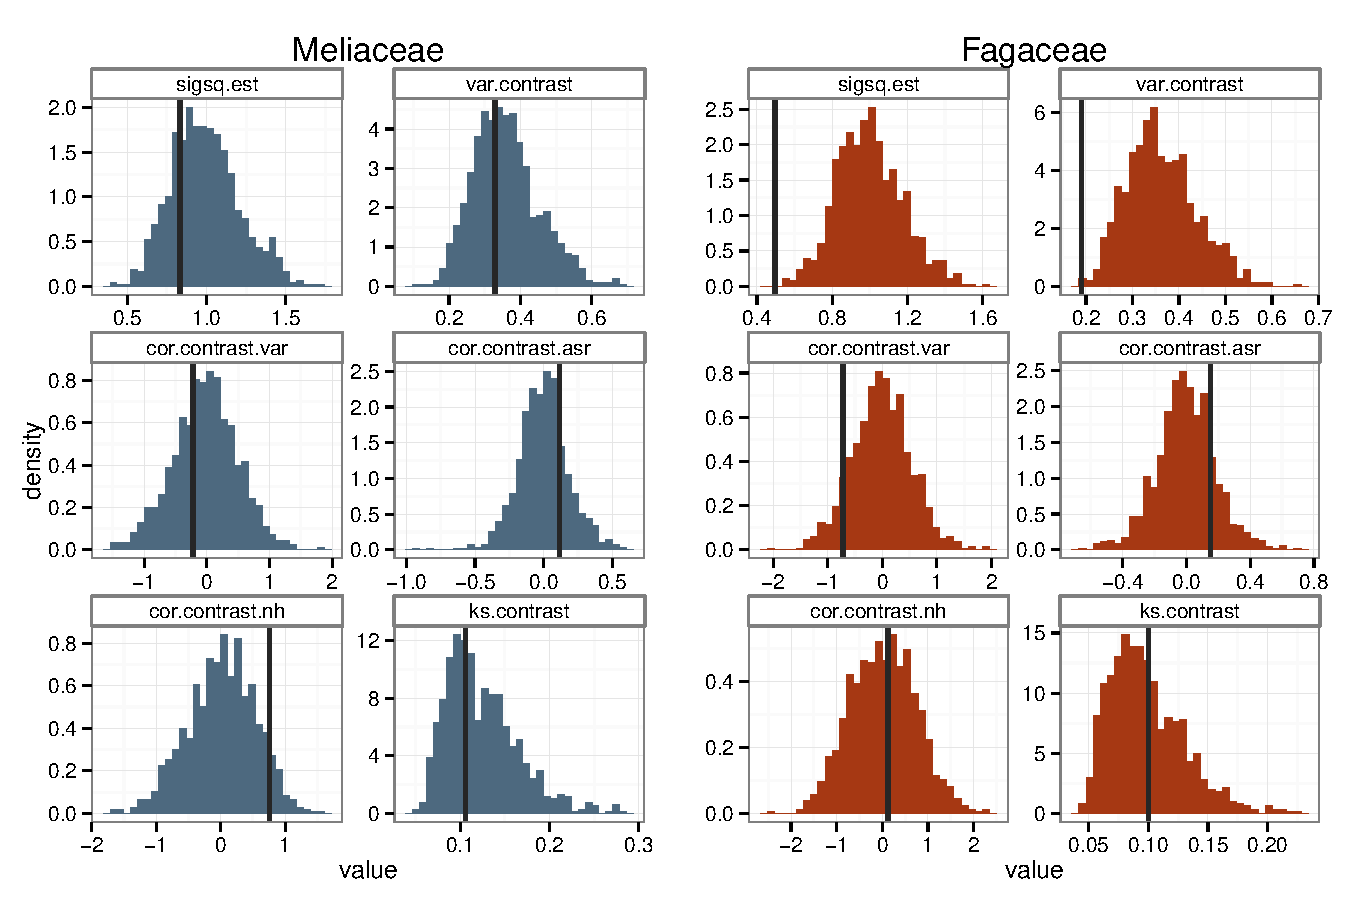
\includegraphics[scale=0.65]{figs/two-clade-example}
  \caption{To be added.}
  \label{fig:two-clades}
\end{figure}

\begin{figure}[p]
  \centering
  \caption{Big fancy tree figure}
  \label{fig:angio-phylogeny}
\end{figure}

\begin{figure}[p]
  \centering
  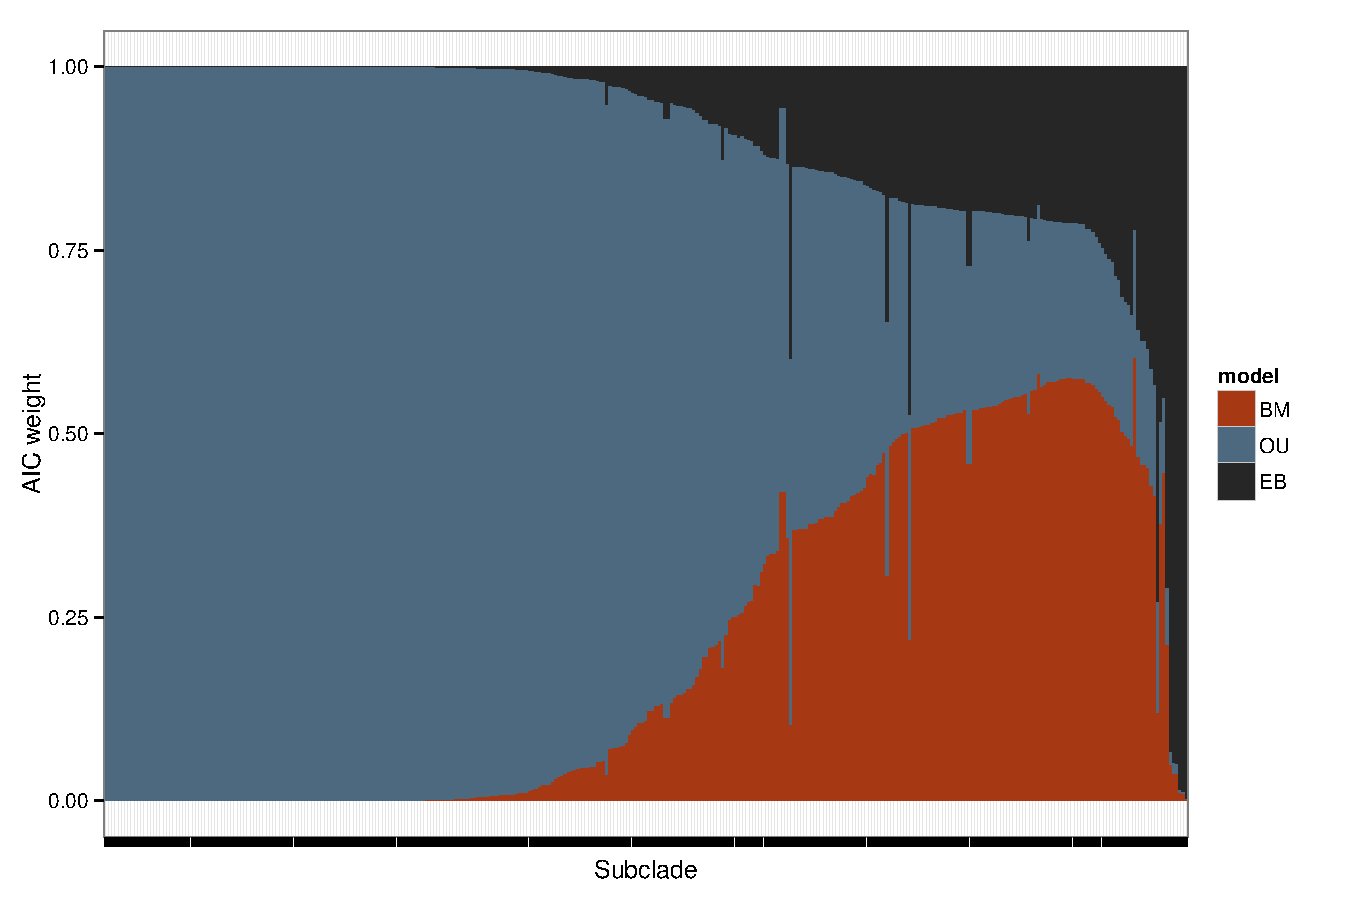
\includegraphics[scale=0.7]{figs/AIC-support}
  \caption{aic support}
  \label{fig:aic-support}
\end{figure}

\begin{figure}[p]
  \centering
  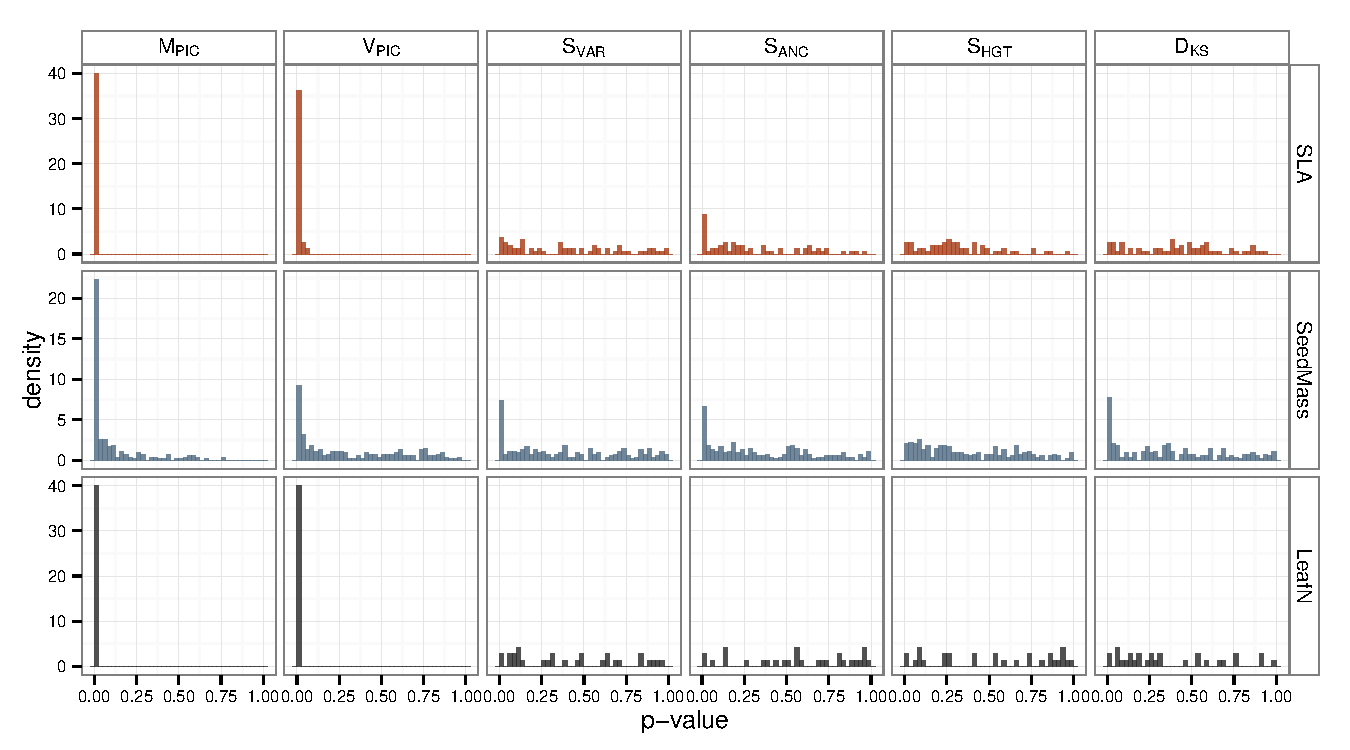
\includegraphics[angle=90, origin=c]{figs/pvalue-hist-ML}
  \label{fig:pvalues}
\end{figure}

\begin{figure}[p]
  \centering
  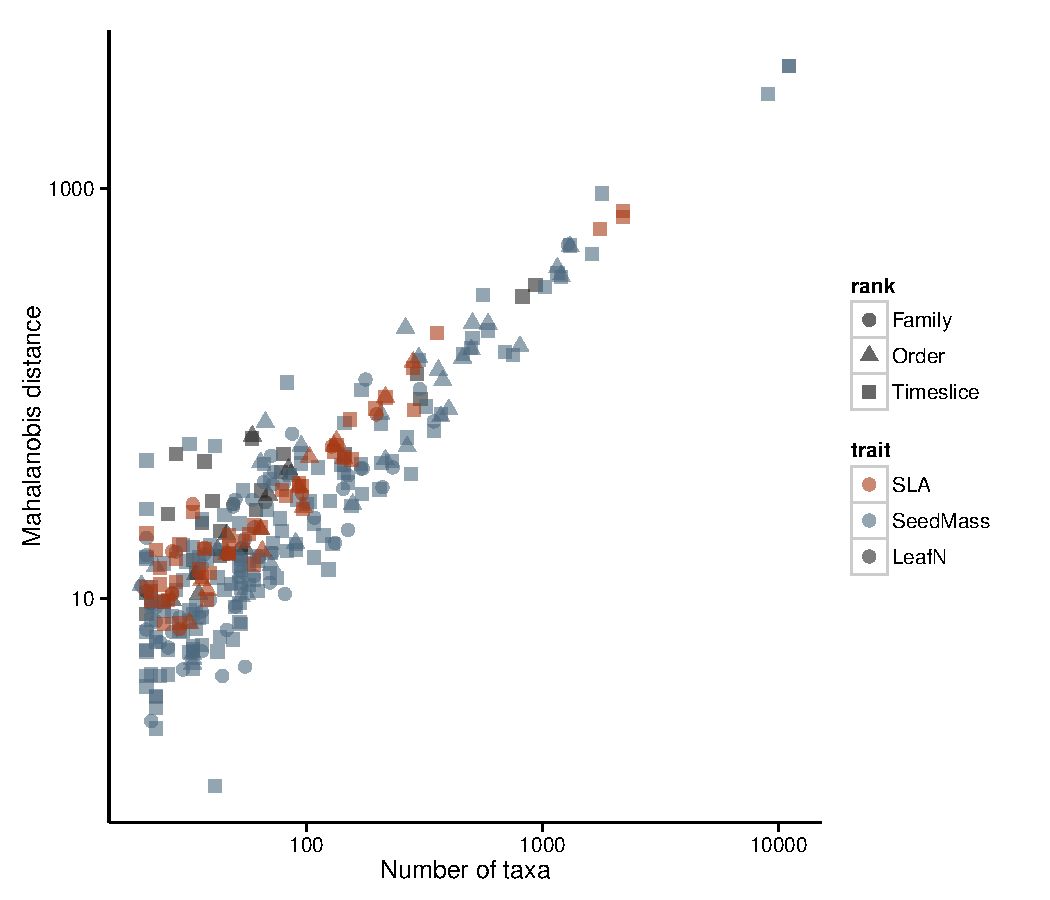
\includegraphics[scale=0.9]{figs/Size-adequacy-ML-bestonly}
  \caption{adequacy v. size}
  \label{fig:size-adequacy}
\end{figure}



\end{document}


